% This is LLNCSDE2.TEX, a variation of LLNCS.DEM
% (the demonstration file of
% the LaTeX macro package from Springer-Verlag
% for Lecture Notes in Computer Science,
% version 2.2 for LaTeX2e),
% which can be used by volume editors for the preparation
% of the front matter pages and the author index
%
% Last changes: 04.08.1999, Antje Endemann (endemann@springer.de)
%
%%%%%%%%%%%%%%%%%%%%%%%%%%%%%%%%%%%%%%%%%%%%%%%%%%%%%%%%%%%%%%%%%%%%%
% In order to generate an Author Index do the following:
% After TeXing this document start the program MakeIndex by typing
% MAKEINDX -S SPRMINDX.STY <filename>
% (generates an IND file for the Author Index)
% into the DOS command line.
% (At other systems you may have to use the command MAKEINDEX.)
% Now TeX this file once again, then you will get an Author Index.
% TeX this file once more, then the TOC will be complete.
%%%%%%%%%%%%%%%%%%%%%%%%%%%%%%%%%%%%%%%%%%%%%%%%%%%%%%%%%%%%%%%%%%%%%

\documentclass{llncs}
%\usepackage{ucs}
\usepackage[utf8]{inputenc}
\usepackage{fancyhdr}
\usepackage[dvips]{graphicx}
\usepackage{graphicx}
\usepackage{fancyhdr,epsfig}
\usepackage{a4wide}
\usepackage{amssymb}
\parskip 3ex



\begin{document}

\title{A comprehensive design model for integrating
learning  processes in e-learning context-aware web applications}

\author{Alejandro Sartorio\inst{1,3}, Griselda Guarnieri\inst{1,2}, Guillermo Rodriguez\inst{1,3}, Patricia San Martin\inst{1,2}}

\index{Ekeland, Ivar}
\index{Temam, Roger}
% use the command \index{<name>} for index entries

\institute{UNR Universidad Nacional de Rosario \and CONICET \and  Agencia}

\maketitle


\begin{abstract}
Web applications have evolved from simple read-only e-learning websites to
complex data- and operation-intensive systems. The main goal of this kind of
application is to provide the users with services (throught the tools as wiki, forum, lessons, etc.) that assist them in carrying out activities according to a given set of pedagogical rules. The addition Obra Abierta requirement to e-learning web applications poses new challenges, such as the managing the
interplay between pedagogical process execution and navigation, and improving
the user’s experience in accessing the services that the e-learning web application offers.
This paper presents a comprehensive design model for integrating pedagogical
processes in e-learning applications focused in the relation between essential object entities (in this case, Students, Teachers and Tools).The model is based on DRObAb, an extended
and revised version of the Ubiquitous Web Applications (UWA) Transaction
Design model for designing web transactions. UWAT+ROA makes it possible to
design e-learnig web application pedagogicaltransactions according to the user’s context and to
integrate the e-learnig web transaction design with the information and navigation design
of the web application.
\end{abstract}


\section {Introducción}

Según San Martín et. al. \cite{libro}, un  Dispositivo Hipermedial Context-Aware Dinámico (DHc-aD) es ....


En este contexto, una transacción (o transacción e-learning) es definida como una secuencias de actividades que el usuario ejecuta a través de la aplicación e-learning con el propósito de efectuar una tarea o concretar un objetivo. El conjunto de actividades, sus propiedades y las reglas que goviernan sus ejecuciones dependen del PEI que la aplicación debe brindar.

Las características tecnológica de un DHc-aD son idénticas a las aplicaciones e-learning convencionales (por ejemplo, las utilizadas en el proyecto de e-learning Sakai) que proveen:  navegación etre páginas a través de links, ejecución de transacciones e-learning por medio de los servicios de las herramientas y las operaciones de un PEI. La principal diferencia tecnológica entre un DHc-aD y una aplicación e-learning convencional es la incorporación de la teoría de coordinación de contratos \cite{fiadeiro, sartorio} en la implementación de algunos servicios que las herramientas brindan a los usuarios \cite{libro}.

Desde el punto de vista de la ingeniería de software, desatender o resolver incorrectamente la documentación para el diseño de procesos de educación e investigación pueden causar numerosos prolemas reflejados en el proceso de configuración  de un DHc-aD. Estos problemas pueden ser:


\begin{itemize}
	\item Dificultades en la comunicación y entendimiento entre los clientes y diseñadores expertos en educación (primero), y entre los diseñadores y los desarrolladores (después), en el proceso de implementación de un DHc-aD.

	\item Determinación de las relaciones donde se justifique la inclusión de contratos.
	
	\item Visualización y caracterización de la conformación de las "redes" de apendizajes e investigación que conforma el Dispositivo \footnote{nota al pié sobre redes de aprendizaje ....}.
\end{itemize}



Este trabajo presenta un diseño compresivo para el modelado de los procesos de educación e investigación (PEI) en un dispositivo hipermedial context-aware dinámico (DHc-aD) \cite{libro}. El modelo está basado en UWAT+ (Distante, 2004), una versión extendida y adaptada de UWA Transaction Design Model para el diseño de transacciones en aplicaciones Web  


..... nos focalizaremos en las transacciones que implementen procesos y que tengan asociada un contrato.

.... hay diferentes tipos de modelos, nosotros nos centraremos en las extensiones para poder implementar la teoríade coordinación de contratos...

..... Teniendo en cuenta nuestra experiencia en el trabajo multidiciplinario de Obra Abierta

..... En este trabajo se retoma el modelo UWAT+ con pequeñas modificaciones 

..... con un pequeño agregado para la extensión del modelo 

....... referenciar a que tipo de modelo corresponde este modelo.

.......  a través de este trabajo mostraremos un simple ejemplo para ilustrar las caractéristicas del modelo de diseño DRObAb 

.......  muy importante para la gente blanda tener un modelo de esta características

....... proponemos una adaptación de la definiciones de colección, slots, etc para educación 


La principales contribuciones de este paper son:

\begin{itemize}
 \item El acercameinto de un modelo útil para la represetación de transacciones e-learning en un DHc-aD. 
 \item Permite una mejor distinción de la ubicación (entre servicio-usuario(s) y servicio-servicio(s)) de la componente contrato dentro del flujo de ejecución.

\end{itemize}

El resto de este paper se encuentra organizado de la siguiente manera: Sección \ref{s2}



\section{Contatos context-aware para tranacciones e-learning}


6.3.2. Coordinación de contratos
En términos generales, la coordinación de contratos es una conexión establecida entre un grupo de objetos (en nuestras consideraciones, un objeto cliente y un determinado servicio serían los participantes), donde reglas, normas y restricciones (RNR) son superpuestas entre los actores participantes, estableciendo con un determinado grado de control las formas de interrelación (o interacción). 
El tipo de interacciones establecidas entre las partes es más satisfactoria que las que se pueden lograr con UML o lenguajes similares (Orientados a Objetos) debido a que éstas contienen un mecanismo de superposición donde se toma como argumento los contextos. Cuando un objeto cliente efectúa una llamada a un objeto suministro, el contrato "intercepta" la llamada y establece una nueva relación teniendo en cuenta el contexto del objeto cliente, el del objeto servidor e información relevante (a la relación) adquirida y representada como contexto del entorno. Como condición necesaria, la implementación de los contratos no debe alterar el diseño y funcionalidad en la implementación de los objetos.


\subsection {Elementos de la componente contrato}

La componente contrato es la información que se tiene de una componente. El contrato puede ser configurado por medio de diferentes mecanismos, desde el lenguaje cotidiano hasta un lenguaje de especificación formal y un lenguaje basado en XML1 para los casos que sean necesarias especificaciones que puedan ser procesadas por máquinas. 
El tipo de tecnología y forma de implementación de los contratos es transparente para los objetos que consumen los servicios en donde se encuentran involucrados.
La configuración de un elemento contrato que forma parte de  las componentes de un servicio, representa la información necesaria del mismo para ser utilizado por el invocador, sin necesidad que el objeto invocador tenga detalles de la ejecución.
El contrato representa una enriquecida y efectiva interface de construcción que contiene toda la información sobre las componentes de los servicios y deberá tener información sobre algún tipo de información de contexto para su utilización.
El concepto de interface en este caso, tiene mayor significación que un simple acceso a un contrato de reglas entre el objeto proveedor del servicio y el objeto consumidor.
En la figura 6.2. podremos observar, los elementos conceptuales básicos de esta componente a través de una serie de elementos en relación con el contrato; este meta-modelo tiene las características conceptuales y operativas que se fundamentan en Obra Abierta. 




\begin{figure}[!h]
\begin{center}
		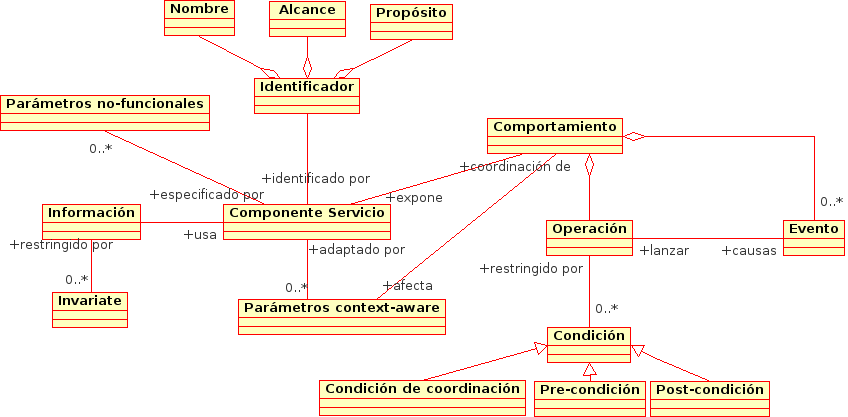
\includegraphics[width=5in,totalheight=2in]{contratoca.png}
                \caption{\small \sl Meta-modelo del contrato context-aware} \label{requerimientos}
\end{center}
\end{figure}
 



Para una mejor comprensión de las componentes del modelo explicitaremos a continuación su caracterización y funciones particulares: 

\textit{Identificador} – Una componente servicio es identificada para un determinado contexto por un único nombre en el espacio de nombre.

\textit{Comportamiento} -  De acuerdo con los roles asignados en un determinado contexto, una componente servicio expone comportamientos correspondientes a provisión y pedido de operaciones, y/o publicaciones y recepción  desde/hacia cada contexto. Las operaciones pueden ser definidas en dos tipos – operaciones que ejecutan cómputos o transformaciones (tipo “update”) y operaciones que proveen algún tipo de información sobre consultas  (tipo “query”). Estas, se encuentran enteramente especificadas en base a  un contrato, con el uso de pre-condición, post-condición y condicionales para lograr la coordinación entre contratos. En las condiciones de coordinación se especifican cómo requerir y proveer operaciones, así como también los eventos publicados  y recibidos son coordinados en los momentos adecuados. Para lograr una comunicación precisa con una componente servicio, no sólo se tiene en cuenta qué operación fue provista o requerida y cómo el ejecutor ha lanzado el evento apropiado, sino también, cómo todas esas actividades están mutuamente relacionadas para ser aprovechadas por el objeto consumidor. Un evento del contexto que lanza una operación dada, puede ser parte de un conjunto de pre-condición, mientras que un evento emitido a través de una exitosa operación puede ser parte de una pos-condición. 
Las operaciones provistas y requeridas por la componente de servicio deben estar asociadas, a fin de determinar las operaciones que deben ser completadas antes de la activación de un servicio (qué es posible de ejecutarse en paralelo o ser sincronizado por otro camino). Por ejemplo, en el caso de una componente de servicio ManegadorOrden, la operación HacerOrden no puede ser invocada hasta que el servicio que la consume no esté correctamente autorizado por el componente de servicio AdministradorRegistros, o la operación deleteOrder no puede ser invocada si la operación HacerOrden con el mismo parámetro OrdenID no fue previamente completada.

\textit{Tipos de Información} –  Una componente de servicio debe  manejar, usar,  crear o tener cierta información de recursos con el propósito de proveer servicios adecuadamente.  Este elemento del contrato define el tipo de información relevante para las componentes  asociadas al contrato, así como también restricciones y reglas sobre instancias de esos tipos. Esto representa un modelo de información lógica de una componente de servicio. Formalmente, esta información de tipos puede ser considerada como definiciones de tipos de  los parámetros de las operaciones o tipos relacionados a ellos.

\textit{Configuración de Parámetros Context-Aware} – Una componente servicio depende del contexto de su actual entorno. La misma, para utilizarse en diferentes contextos logrando la adaptación a eventuales cambios debe tener definido un conjunto de parámetros de configuración.  Ejemplos de estos parámetros pueden ser: Contexto-del-Usuario (CU) - en un sentido similar a lo definido en el capítulo anterior, locación en tiempo y espacio de los servicios consumidos y suministrados. Estos parámetros, pueden ser enviados dentro de las invocaciones de las operaciones de los servicios o por medio de otros caminos, mediante componentes de servicios que pueden adaptar su comportamiento ante el cambio de contexto en una determinada situación.  
La configuración de parámetros está directamente asociada a las relaciones de las operaciones de los servicios para lograr una mejor adaptación a la medida de las circunstancias brindada por la información relevada del contexto. El concepto de la configuración de los parámetros context-aware, es un paso muy importante hacia la concepción de servicios automatizados y auto adaptables (tomando el sentido paradigmático de los teóricos de la Inteligencia Artificial).

\textit{Parámetros no funcionales} – Una componente servicio puede definir un conjunto de  los llamados parámetros no funcionales que caracterizan a la “calidad” de sus prestaciones dentro de un determinado contexto. Estos parámetros, son elementos para los consumidores de los servicios que permiten optar por el uso de un determinado  servicio, o buscar otro con el mismo o similar contrato. Como ejemplo de parámetros no funcionales podemos mencionar: Performance, Fiabilidad, Tolerancia a Fallos, Costos, Prioridad y Seguridad.




\section{Documentación de los procesos de educación e investigación}


Las transacciones e-learning en un DHc-aD están definidas como secuencias de actividades asociadas con un flujo de ejecución que permite al usuario desempeñar una determinada tarea  y/o alcanzar una meta a través del dispositivo hipermedial. Entonces, un porceso de educación e investigación puede ser interpretada como una especificación del concepto de "workflow" en una aplicación e-learning Web, con las condiciones (restricciones) que implica la concreción de un PEI.


En una transacción e-learning Web, una  $Actividad$ está  conformada por un conjunto de operaciones simples o complejas sobre datos y contenidos de la aplicaciones e-learning. Como ejemplo de transacciones e-learnign se pueden mensionar un proceso en el cual un usuario (p. ej., un alumno) participa en un espacio de edición colaborativa (este caso será analizado posteriormente bajo la metáfora de la mesa de arena \footnote{mesa de arena}) 

Entonces, las transacciones en un DHc-aD son el camino para la representación de los PEI y proveer a los usuarios de servicios accediendo a través de las herramientas que los contienen (wiki, foro, video conferencia, taller, blog, etc.) La ejecución de transacciones de un DHc-aD supone tanto la navegación a través de las herramientas (por medios de los links de las componentes hipermediles) como  el uso de sus servicios. Un ejemplo de servicio puede ser en una video conferencia la posibilidad de que un docente edite en una pizarra compartida (con sus alumnos y colaboradores) una determinada ponencia. 

El diseño de las transacciones  abarcar varios niveles de abstracción, distintos formalismos pueden ser usados para su representación y documentación. Al menos tres nivels de abstracción pueden ser representados: (1) nivel conceptual, (2) nivel lógico, y (3) nivel de implementación.  El diseño conceptual permite una representación del sistema (las transacciones y su alcances) tal cual son persividas por el usuario despejando las cuestiones de implementación. El diseño de la implementación se encuentra focalizado a proveer a los diseñadores de los DHc-aD con todas las especificaciones necesarias para la configuración y realización de sus componenetes. El diseño lógico es un nivel intermedio del diseño de abstracción con la intención de trasladar las especificaciones centrales del usuario desde el diseño conceptual en terminos de  especificaciones más cercana a las implementaciones.

Al igual que lo que ocurre con todos lo artefactos de software, el diseño de una Transacción e-learning para un DHc-aD  se puede tornar muy complejo. Cuanto más complejo sea el diseño, las confusiones entre los diseñadores (expertos en educación)  y los implementadores (Web master, encargado de la plataforma) crecerán. Para comunicar efectivamente la idea del diseñador es necesario una apropiada documentación. La documentación textual ha sido muy utilizada para describir detalles de implementaciones de bajo nivel. Teniendo en cuenta que el diseño de las transacciones e-learning se describen en un  nivel conceptual, es más adecuado una representación gráfica. 

Existen diferentes aportes  directamente relacionado a modelos "visuales" en forma de documentación gráfica \cite{5,10,12}. En este contexto los modelos visuales son representaciones de systemas de software que soportan multiples perspectivas. Para el caso del diseño de las transacciones e-learning, una vista puede ser representada por una series de diagramas pertenecientes a UML (Unified Modeling Language) 

Los antecedentes relevantes que se relacionan con lo que entendemos por diseño de PEI, fueron estudiados de los aportes del campo del métodos de diseños para aplicaciones Web experimentados en los últimos años. Concretamente se pueden mensionar ADM (Atzeni y Parente, 2001), OO-H (Koch et al., 2003), OOHDM (Schmid and Rossi, 2004) y UWAT+ 

UWAT+ es un meta-modelo para la descripción de los distintos aspectos de Transacciones Web de manera holística. Es una extensión del Modelo de Diseño de Transacciones que es parte del framework UWA (Ubiquitous Web Applications). Inspirado en este modelo y extendiendolo para la contensión de los contratos, se describe una adaptación para el diseño de transacciónes e-learning en un DHc-aD.

\section {DRObAb: una adaptación de UWAT+ para el modelado de PEI en DHc-aD}

Si bien los métodos de diseño de transacciones de UWAT+ pueden ser utilizados para la representación de transacciones e-learning, es necesario efecutuar adecuaciones que tengan en cuenta  a los contratos. Tal cual fue mensionado en la sección \ref{introduccion}, desde la perspectiva de los diseñadores, los contratos deben ser visto como una pieza de software para mejorar la instrumentación de los servicios de las herramientas. En consecuencia, es necesario tener un modelo que permita una mejor representación de los contratos, la visualización de su inserción en los servicios y las relaciones que en ellos representan. 


La figura \ref{drobab} se muestra un diagrama de clase UML que representa a los conceptos, las relaciones entre conceptos y los modelos para la representación de transacciones. Los esquemas en color blanco pertenecen al modelo original UWAT+. El rectángulo y los esquemas grices describen los objetos, modelos y relaciones que fueron que conforman DRObAb.


	\begin{figure}[!h]
        \begin{center}
	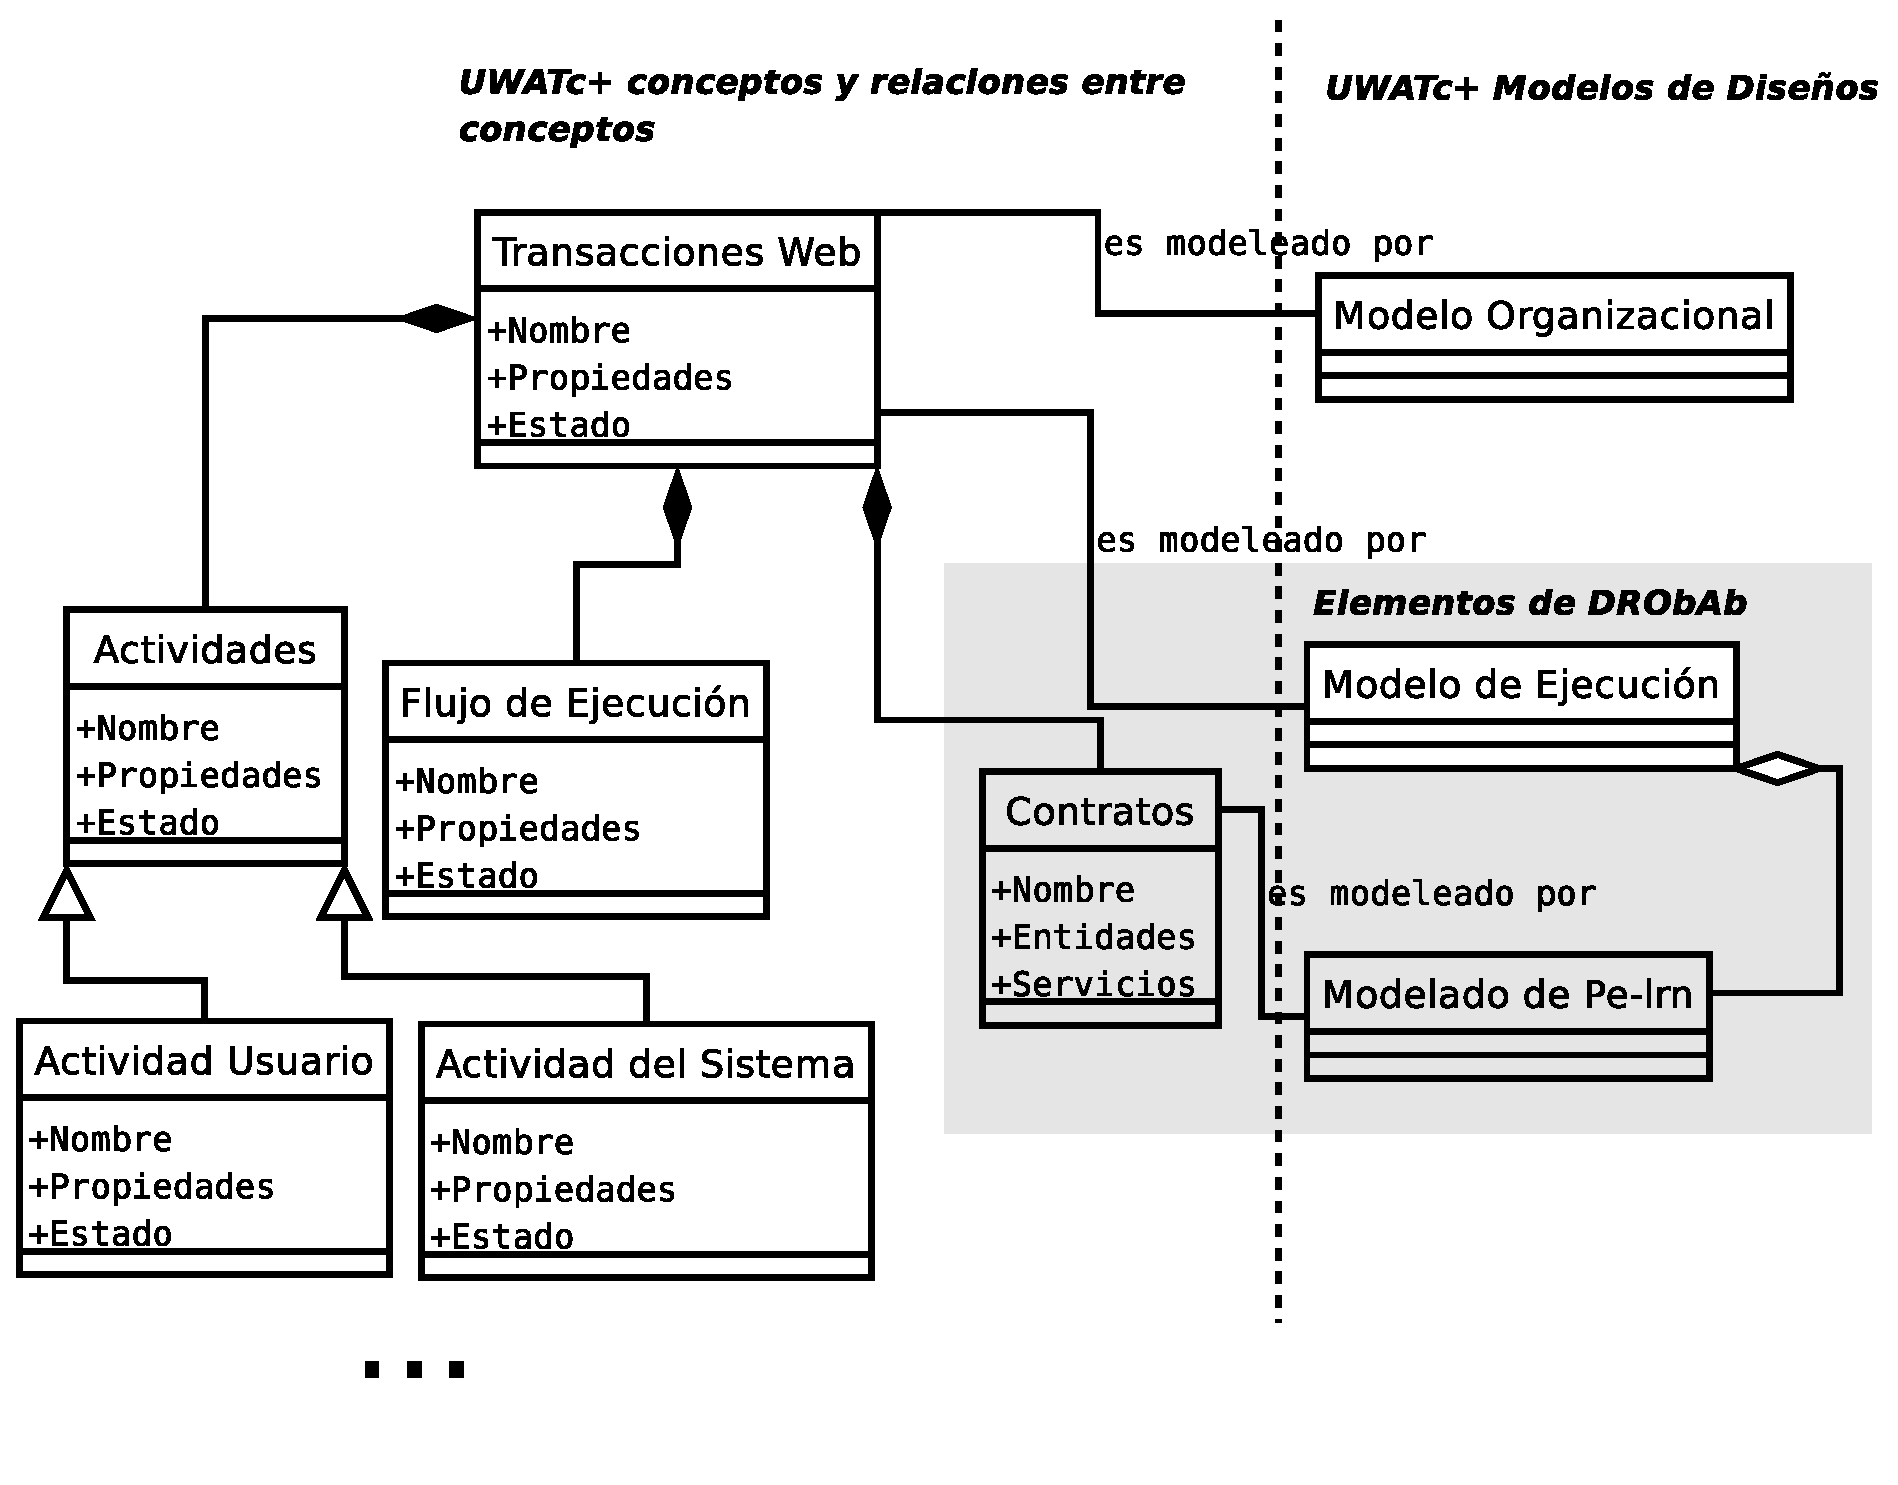
\includegraphics[width=5 in,totalheight=3 in]{drobab.eps}
	\caption{\small \sl DRObAb modelo conceptual y de diseño} \label{drobab2}
         \end{center}
         \end{figure}


Como se describe en el diagrama, una transacción web es un objeto complejo (concepto) compuestos por dos tipos de objetos principales pertenecientes al modelo original de UWAT+ y un tercer objeto  agregado para la representación de los contratos pertenecientes a las transacciones e-learning. En el primer grupo se encuentra $Actividad$ para la distinción de las actividades de los usuarios y del sistema. El objeto $Flujo de Ejecución$ representa del órden lógico y temporal para la ejecución de las actividades comprendidas en las transacciones. A su vez, una transacción web puede ser descripta por el $Modelo Organizacional$ (desde el punto de vista estático) y el $Modelo de Ejecución$ para la definición de las reglas de ejecución de la componente actividad (desde el punto de vista dinámico). 

Cuando una transacción web contiene un contrato (definida como transacción e-learning) debe ser incluida una nueva componente para el diseño (representrada en la figura como una relación de agregación en el $Modelo de Ejecución$), conjuntamente con un nuevo modelo de diseño, $Modelo de PEI$, que permite representar al contrar (caracterizada con la asoción con el objeto $Contrato$).

De esta manera quedan conformados los elementos que componen el modelo DRObAb (rectángulo gris) y sus relaciones con el modelo original UWAT+. La sisguiente sub-sección describe en detalle el modelo usado por DRObAb para el diseño de los mensionados contratos  


\subsection{Requerimientos para el diseño de trasacciones e-learning}

En esta sección se describen la caracterización de dos tipos representativo de requerimiento que motivaron la creación de este nuevo modelo de diseño de los PEI (definidos en la sección \ref{sección1}). En base a experiencias recogidas - por el grupo Obra Abierta \footnote{Obra Abierta: } -  en el diseño y configuración de herramienta e-learning, se presentarán dos tipos de requerimientos que deben ser cubiertos por el diseño. En primer lugar se enuncian cuestiones técnicas de diseño (desde el punto de vista de la Ingeniría de Software), seguido de un comentario sobre que tipo de transacción que el diseñador puede especificar a través del diseño

En esta sección se describen la caracterización de los requerimientos que motivaron la creación de este nuevo modelo de diseño de los PEI (definidos en la sección \ref{sección1}). En base a experiencias recogidas - por el grupo Obra Abierta \footnote{Obra Abierta: } -  en el diseño y configuración de herramienta e-learning, se presentarán dos tipos de requerimientos represetativo. En primer lugar se enunciarán cuestiones técnicas de diseño (desde el punto de vista de la Ingeniría de Software), seguido de un comentario sobre los elementos de la transacción resaltados por el diseño y sus relaciones (desde el punto de vista del diseñador).

\begin{itemize}

\item Especificar como son afectadas la ejecución de las actividades por los objetos contratos. 
\\

La relación de una actividad con un contrato se produce cuando existen objetos interrelacionados con un contrato \cite{interconecting}. De esta manera, el diseñador debe porder documentar las información de los objetos involucrados (métodos y parámetros). El contrato representa un tipo diferente de relación a la origianal (entre los objetos), con un carácter más volátil y mejor orientada a las características de las transacciones e-learning.



Cada vez que una actividad esté relacionada con un contrato, 


La relación de un contrato con una actividad se produce a través de la interconexión entre objetos por medio de un contrato.





\item  Definir cual y como la  información de los objetos contratos ("information object" \cite{information_object}) es afectada por la ejecuticón de las actividades.
\\

Una actividad funcional conciste en la ejecución de uno a más operaciones elementales (inserción, borrado, modificación, etc.) sobre la datos de la aplicación y la información de los objetos contratos envuelta en la actividad. El modelo de diseño de transacciones e-learning debe permitir al diseñador definir cuales operaciones del contrato son fundamentales para cada actitividad, modelando el camino en que cada actividad elemental afecta la información de los objetos involucrados (modificando sus instancias por medios de sus ejecuciones).


\end{itemize}


\subsection {Modelo para PEI}


\section {Diseño de procesos de Educación e Investigación con DRObAb}

En esta sección se describen los resultados de la apliación de DRObAb para el espacio dedicado al libro "Hacia un dispositivo hipermedial contex-aware Dinámico. Educación e investigación para el campo audiovisual interactivo" (San Martín P, et. al) \cite{libro}.  Este  modelo fue aplicado parcialmente para el diseño de los requerimientos fundamentales y el modelado del compertamiento funcional enmarcado bajo la perspectiva de Obra Abierta \cite{ObraAbierta}. Se identificarán las ........

El diagrama de la figura \ref{procesodiseno} muestra una adaptación del diseño de procesos de UWA \cite{UWA} que se utiliza en DRObAb para el diseño de los PEI. Para ilustrar el proceso de diseño se utiliza IDEF0 (IDEF-0, 1993). A continuación, se describen las fases que fueron adoptadas en cuya implicancia se determinen las cuestiones que involucran a los contratos y la caracterización de los PEI significativos de Obra Abierta para \cite{libro7}:

\begin{enumerate}
 \item Determinación de Requerimientos 
 \item Diseño de procesos
 \item Diseño de operaciones
 \item Diseño de navegación
\end{enumerate}

	\begin{figure}[!h]
        \begin{center}
	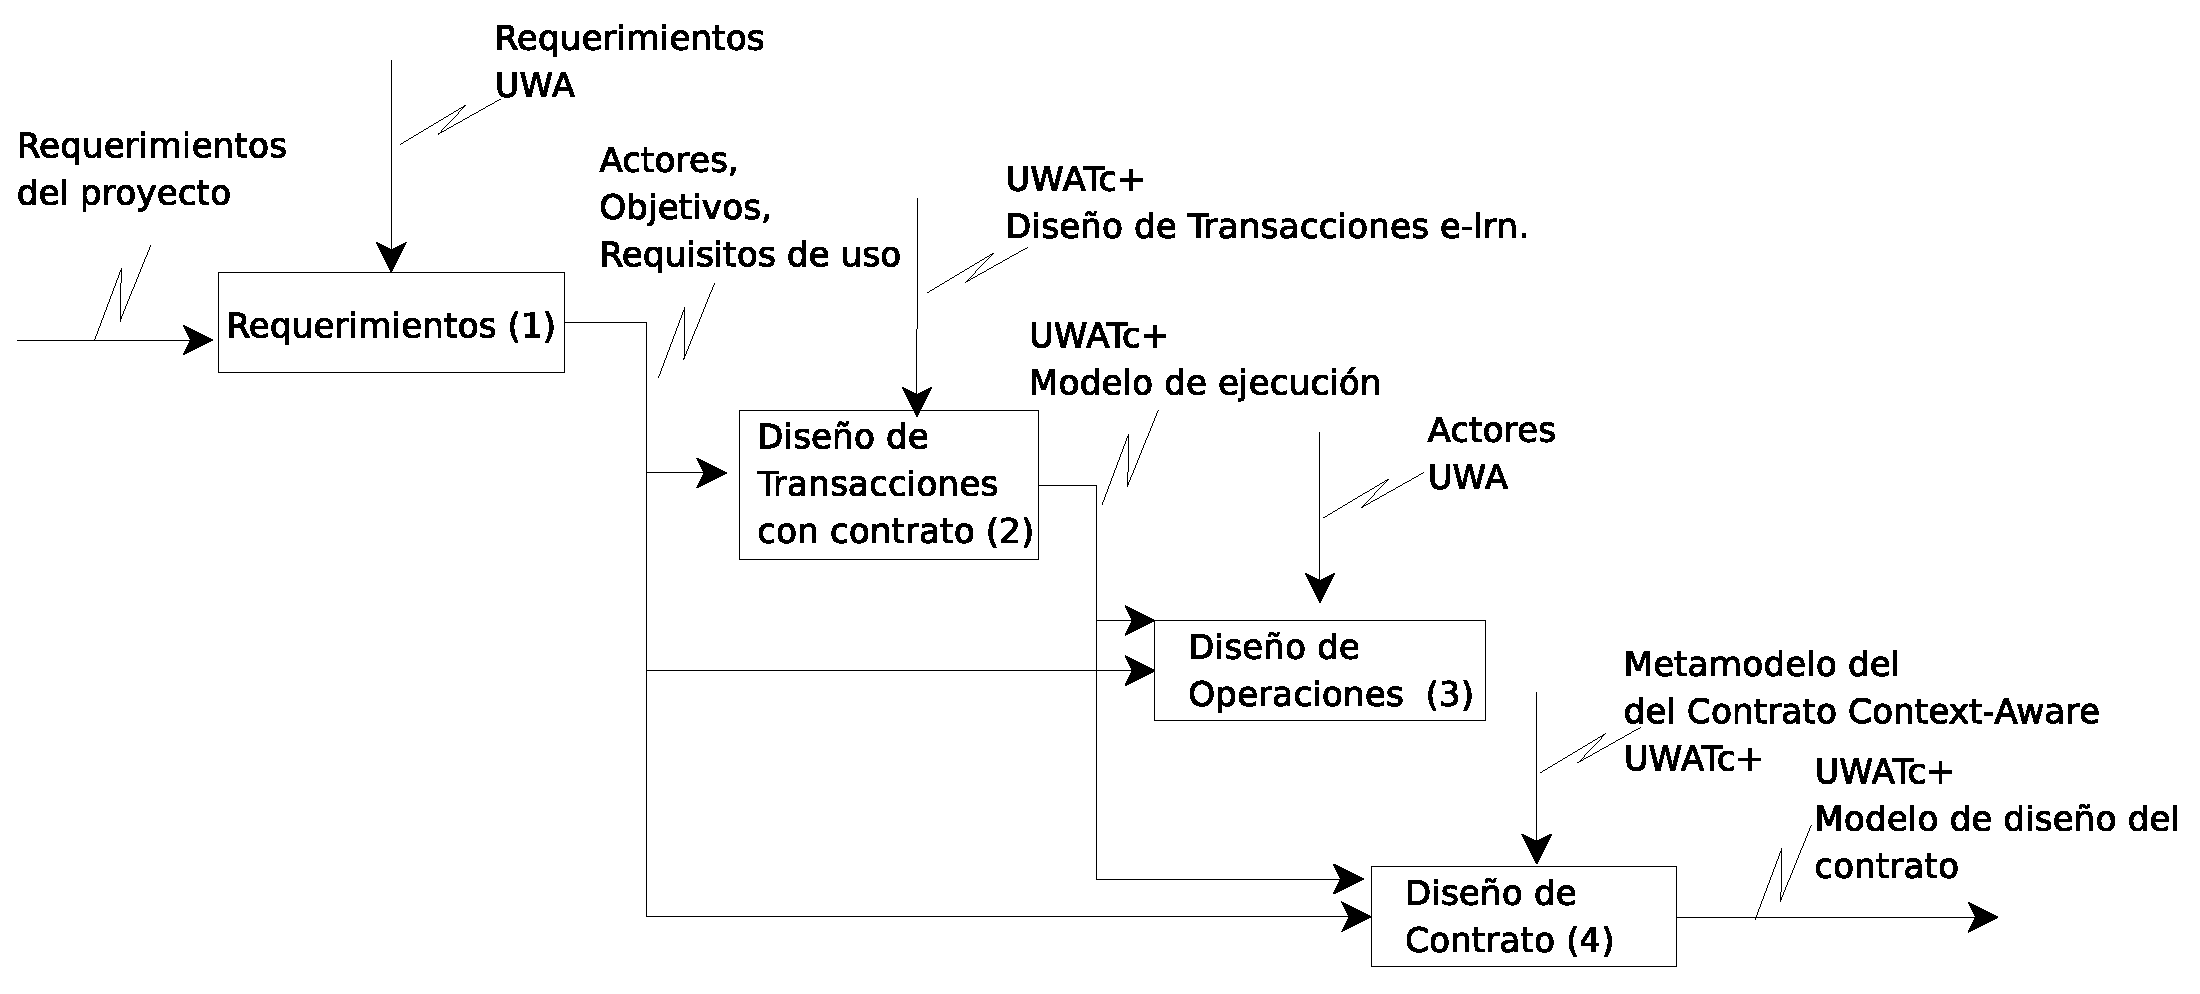
\includegraphics[width=6 in,totalheight=2 in]{procesodiseno.eps}
	\caption{\small \sl El proceso de diseñar PEI en un DHc-aD con DRObAb} \label{proceso de diseno}
         \end{center}
         \end{figure}

\subsection{Determinación de Requerimientos} \label{sdr}

La fase de Determinación de Requerimientos toma como entrada las especificaciones del proyecto y produce, por medio de un mecanismo de refinamiento, las siguientes salidas:
\begin{itemize}
 \item  Cada actor con su objetivos relativos.
 \item  Los requerimientos para el DHc-aD.
\end{itemize}
 
El modelo utilizado es orientado a objetivos: cada actor se identifica con al menos un objetivo, i.e, una abstracción de los objetivos que a través del dispositivo hipermedial se debe alcanzar; cada objetivo es refinado en otros sub-ojetivos, concretando hasta poder definir el requerimiento objetivamente o en un bajo nivel suficiente para poder implementar el requerimiento. Este fase es similar a la descripta en (UWA Consortium, 2001) \cite{UWA}. 

Para este caso de uso, atendiendo a los lineamientos en \cite{libro7}, se descibe parte del modelo original donde se carateriza los objetivos involucrado con un actor relevante del sistema. A su vez, a medida que se van derivando los sub-objetivos comienzan a establecerse requerimientos concernientes a la teoría de coordinación de contratos context-aware \cite{libro5,contratos}. En la figura \ref{requerimientos} dicha situación ocurre en la derivación de las tres ramas de objetivos y sub-objetivos, influyendo directamente en la composición de la componente contrato; tomando desde la \textit{\textbf{rama 1}} un servicio de una herramienta de un espacio de discusión (ejemplo, el foro), de la \textit{\textbf{rama 2}} se despenden las información necesaria para poder articular dicho servicio teniendo en cuenta la información de contexto y, luego,  la \textit{\textbf{rama 3}} aporta el consenso de los expertos (del dominio e-learning) para la inclusión de los contratos en aquellas relaciones que mantendrán las propiedades de un dispositivo hipermedial dinámico context-aware \cite{libro5}. De esta manera, te tienen todos los elementos (caracterizados y formalizados para su compresión) para la confección de los contratos context-aware.

	\begin{figure}[!h]
        	\begin{center}
		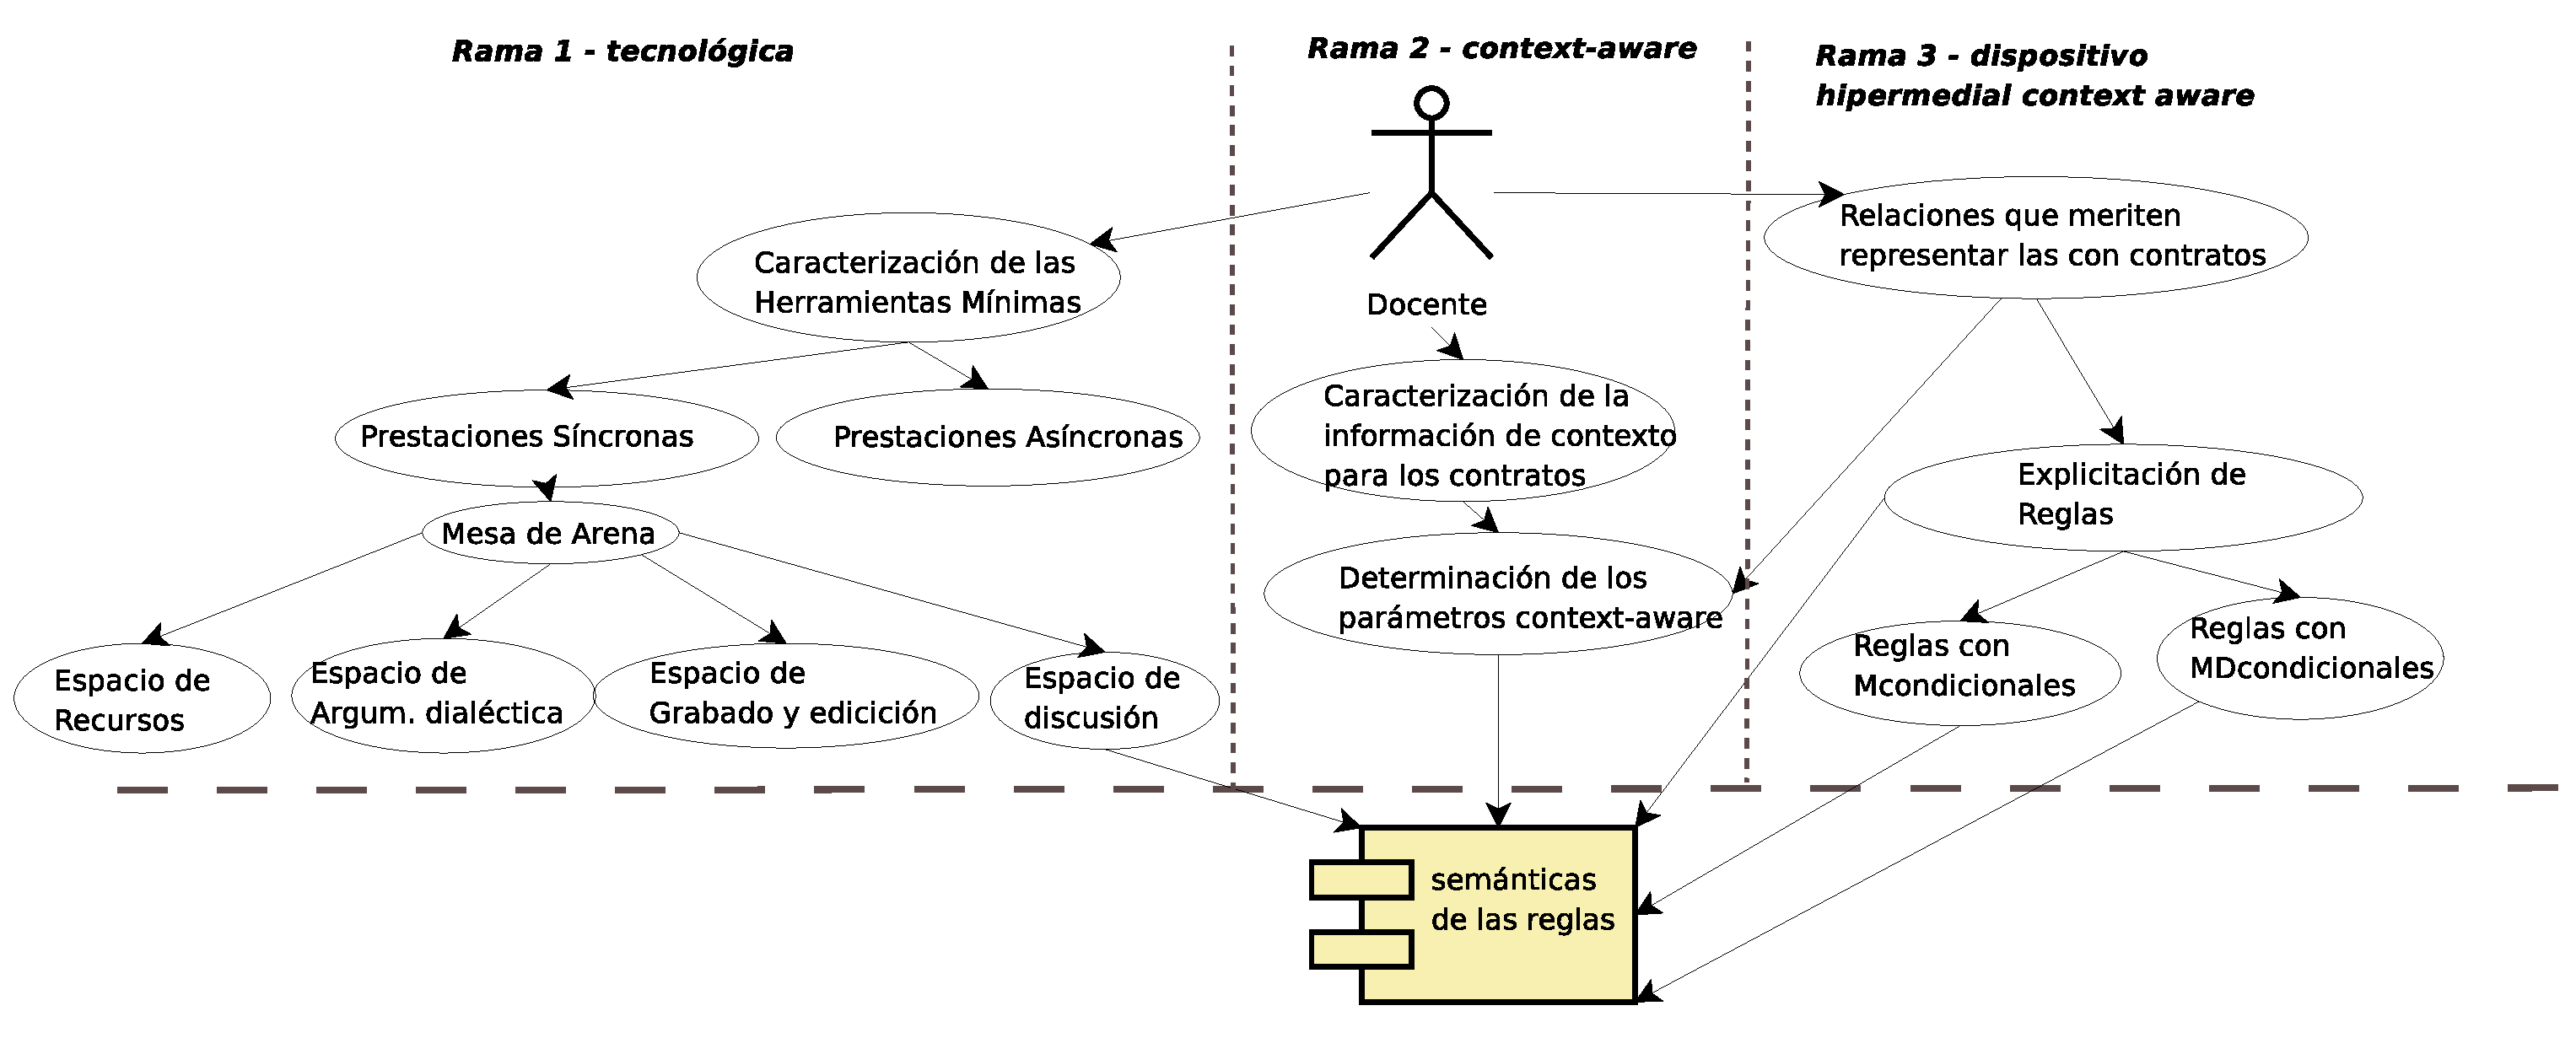
\includegraphics[width= 6 in,totalheight=3 in]{Requerimientos.eps}
                \caption{\small \sl Objetivos de al alto nivel  para el PdEAI} \label{requerimientos}
         	\end{center}
         \end{figure}


\subsection{Diseño del Procesos}

El diseño de procesos retoma la misma idea y modelo propuesto por UWAT+ para el diseño de transacciones \cite{UWA+}. Partiendo de los resultados de los Requerimientos, fundamentalmente de la caracterización de los contratos, pueden ser seleccionados una series de procesos, i.e. objetivos que requieran la ejecución de una o más actividades para su cumplido. Para cada uno de los objetivos deben ser diseñados procesos (el equivalente a las transacciones en UWA+), los cuales en principio deben ser establecidos desde un punto de vista estático (en este trabajo no abordaremos tal consideración) y luego, desde un punto de vista dinámico por medio de un modelo de ejecución de procesos. En la figura \ref{ejecucion de procesos} se muestra una porción del modelo de ejecución de un PEI en donde se usa el contrato modelado en la fase de Determinación de Requerimientos (figura \ref{requerimientos}, sección \ref{sdr}). 

...... por q tomamos la parte dinámica y no la estática ?

\begin{figure}[!h]
        \begin{center}

	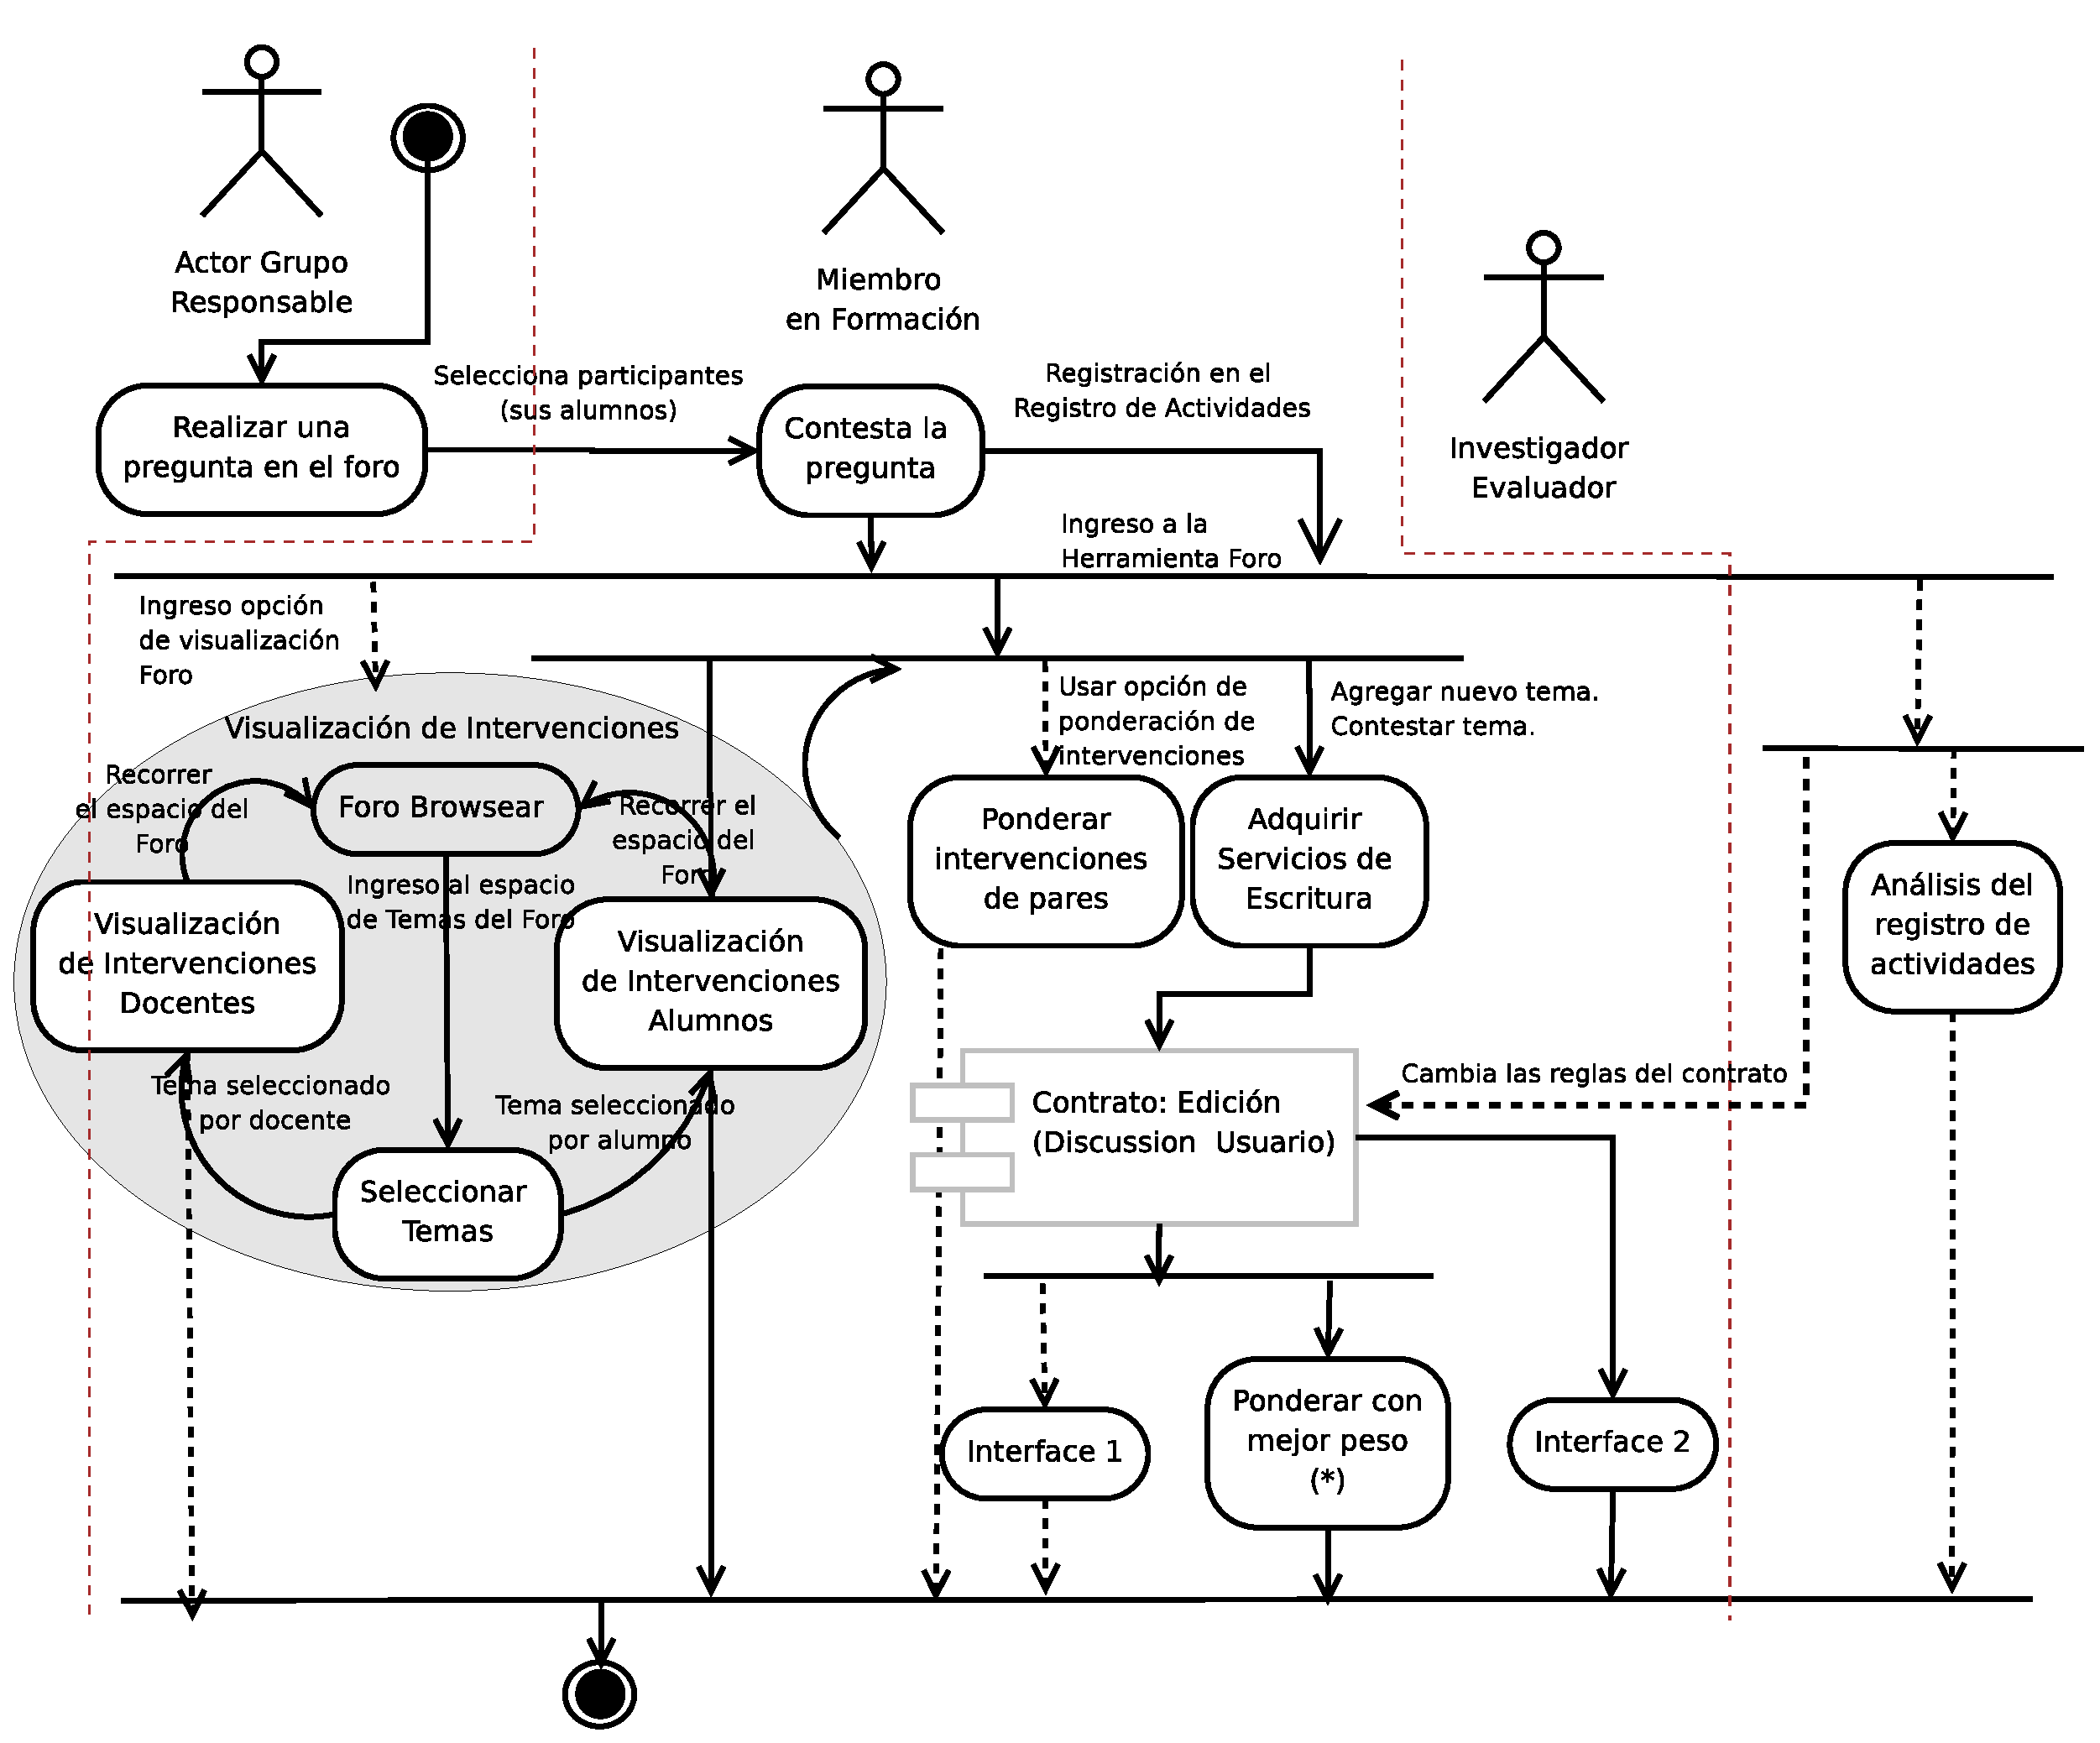
\includegraphics[width= 5 in,totalheight=3.5 in]{proceso.eps}
                                    \caption{\small \sl Modelo de ejecución de Procesos de Educación e investigación} \label{proceso}
         \end{center}
         \end{figure}

\subsection{Diagrama de Contrato para un Pe-lrn}

Existen diferentes formas de representación de los contratos definidos en \ref{contratos}, la herramienta  CED (Coordination Development Environment) \footnote{CED: es el primer prototipo de una herramienta que implementa el uso de la coordinación de contrato en aplicaciones Java. La herramienta pertenece a ATX Sofware (www.atxsoftware.com.ar);fue desarrolada en Java y es de código abierta.} los implementa a través de un lenguaje llamado Oblog \cite{lenguajeoblog}. En \cite{communit} se muestra como a través de CommUnity se definen primitivas de modelado y técnicas de diseño basadas en la separación de la "coordinación" del "cómputo". 

En DRObAb se brinda un diagrama de representación de contrato, donde se describen todos los datos que lo instancian. Cada tipo de dato y valor, pertenece a un elemento del meta-modelo de la figura \ref{modelocontratoca}. En primer lugar (item 1) se identifican los objetos participantes en el contrato; en el ejemplo de la figura \ref{diagramacontrato} DiscussionAction y UserAction hacen referencias a dos clases reales pertenecente al Foro y Usuarios de la herramientra Sakai, respectivamente. Luego, se identifican los nombres de los parámetros context-aware significativos para el contrato, alineados en la misma columna del objeto que lo comparte (item 2). En Servicios (item 3) deben ser represetados los métodos del objeto que al ser ejecutados - eventualmente -  probocan la intervención del contrato, para este ejemplo $initState$ y $getIdentifier$  son ejecutados cuando un usuario ingresa a la herramienta Foro de Sakai y las posteriores funcionalidades dependen de la ejecución del contrato $Edición$ (la figura \ref{procesodiseno} muestra la superposición del contrato entre los servicios de edición y las nuevas interfaces o funcionalidades). Los siguentes filas (items 4 y 5) se refieren a las pre y post condiciones que se deben cumplir en la ejecución del contrato. Por último se explicitan las reglas de coordinación. Siguiendo con el ejemplo, en la parte del condicional $u.contexto=’l1;p1;docente;r1;c1;’$ verifica si el contexto del usuario $u$ está compuesto por la locación $l1$, tienen el perfil $p1$, es un $docente$, cumple el rol $r1$ y pertenece a la categoría $c1$ (este tipo se encuentra desarrollado en \cite{libro}). En cuanto a acción de la regla -continuando con el mismo ejemplo, se induce la ejecución del método $showMessage$ del objeto $d$ (DiscussionAction). El final del diagrama está dedicado a comentarios; cada comentario dede ir acompañado con el número de item (1,2,3,4,5 o 6) al que hace referencia. 




\begin{center}

\small{ 

\begin{tabular}{|l|p{20mm}|p{55mm}|p{1mm}|p{55mm}|} 
		\hline 
\multicolumn{5}{|c|}{\textbf{Contrato:} Edición}\\
		
\hline 
1.& \textit{Participantes}: 	& \textbf{d}:DiscussionAction && \textbf{u}:UserAction \\
\hline 
2.& \textit{Param. c-a}: 	&	state, portlet, rundata, context &&  	context$_$identifier, identifier 	\\
3.& \textit{Servicios}:		& 	initState()		 	 &&	getIdentifier()				\\
4.& \textit{Pre-Cond}: 		& existe $<contexto>$ 			&& existe $<contexto>$  \\
5.& \textit{Pos-Cond}: 		& modifica $<contexto>$ 		&& \\
\hline 
6.& \textit{Reglas      de Coordinación}: & \multicolumn{3}{l|}{{\textbf{Si} \textbf{u}.contexto='p1;d;r1;c1;' \textbf{entonces} \textbf{d}.showMessage(data,string)}}  \\
\hline 

\multicolumn{5}{|c|}{\textbf{Comentario}} \\
\multicolumn{5}{|l|}{4. data: ; string: ; contexto: } \\
\multicolumn{5}{|l|}{fdfdsfdsfdsfdssdsffsddfsdfsdfs} \\

\hline
\end{tabular} 
}
\end{center}


Este modelo es liviano

los prepos condiciones pueden ser tratodos con ocl 

el tema del contexto puede ser modeladocon conte

context base contraint CoCon


\section {Conclusiones}


%-------------------------  bibliografía ----------------------------------

\newpage

\begin{thebibliography}{1}

\bibitem{libro5} Sartorio A., San Martin P., 2007. {Sistemas Context-Aware en dispositivos hipermediales dinámicos para educación e investigación}

\bibitem{libro} San Martín P., Sartorio A., Guarnieri G., De la Riestra M., 2007. {Hacia un dispositivo hipermedial context aware dinámico. Educación e Investigación para el campo audiovisual interactivo}

\bibitem{ObraAbierta} Sartorio A, San Martin P., 2007. {Sistemas Context-Aware en dispositivos hipermediales dinámicos para educación e investigación}

\bibitem {5} Hartmann, J.; Huang, S.; and Tilley, S. {“Documenting
Software Systems with Views II: An Integrated Approach
Based on XML.”} Proceedings of the 19th Annual
International Conference on Systems Documentation
(SIGDOC 2001: October 21-24, 2001; Santa Fe, NM), pp.
237-246. ACM Press: New York, NY, 2001.

\bibitem {10} Tilley, S. and Huang, S. {“Documenting Software Systems
with Views III: Towards a Task-Oriented Classification of
Program Visualization Techniques”.} Proceedings of the 20th
Annual International Conference on Systems Documentation
(SIGDOC 2002: October 20-23, 2002; Toronto, Canada), pp.
226-233. ACM Press: New York, NY, 2002.

\bibitem {12} Tilley, S.; Müller, H.; and Orgun, M. “Documenting
Software Systems with Views.” Proceedings of the 10th
Annual International Conference on Systems Documentation
(SIGDOC ‘92: October 13-16, 1992; Ottawa, Canada), pp.
211-219. ACM Press: New York, NY, 1992.

\end{thebibliography}

\end{document}
